% Source: AESP_466_ClassWork/Supplements/Companion/Euler_Sequences_Quaternions/Euler_Sequences_Quaternions.tex

\documentclass[border=4pt]{standalone}
\usepackage{amsmath}
\usepackage{amssymb}
\usepackage{graphicx}
\usepackage{tikz}
\usepackage{xcolor}
\usetikzlibrary{shapes.geometric, arrows.meta, positioning, decorations.pathmorphing, decorations.pathreplacing, patterns, calc, 3d}

\definecolor{Garnet}{HTML}{73000A}
\definecolor{USC_Rose}{HTML}{CC2E40}
\definecolor{USC_Blue}{HTML}{466A9F}
\definecolor{USC_Slate}{HTML}{1F414D}
\definecolor{USC_Olive}{HTML}{65780B}
\definecolor{USC_Lime}{HTML}{CED318}
\definecolor{USC_Gold}{HTML}{A49137}
\definecolor{USC_Black90}{HTML}{565656}
\definecolor{USC_Black10}{HTML}{ECECEC}

\newcommand{\sectionheader}[1]{%
  \vspace{0.5cm}
  {\noindent\Large \textbf{#1}}
  \vspace{0.2cm}
  \hrule
  \vspace{0.1cm}
  \hrule
  \vspace{0.3cm}
}

\begin{document}
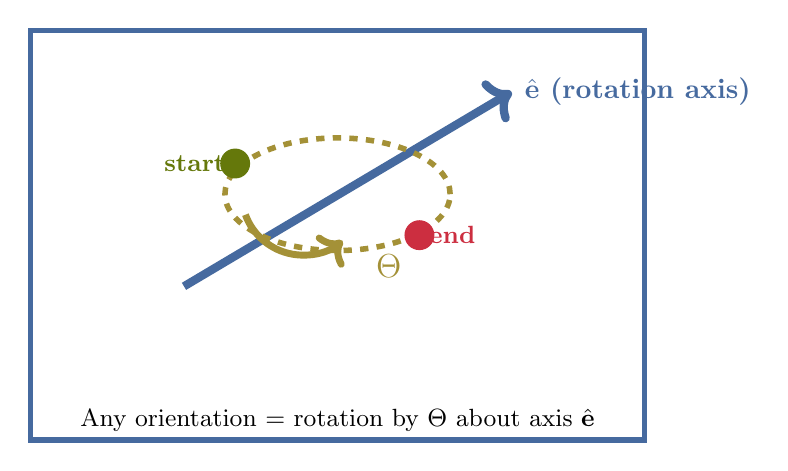
\begin{tikzpicture}[scale=1.3]
    % Border box
    \draw[draw=USC_Blue, line width=2pt, fill=white] (-1.5,-1.5) rectangle (4.5,2.5);

    % Axis of rotation
    \draw[->, line width=3pt, USC_Blue] (0,0) -- (3.2,1.9) node[right, font=\bfseries] {$\hat{\mathbf{e}}$ (rotation axis)};

    % Rotation arc
    \draw[line width=2pt, USC_Gold, dashed] (1.5,0.9) ellipse (1.1 and 0.55);

    % Angle arc
    \draw[->, line width=2.5pt, USC_Gold] (0.6,0.7) arc (200:310:0.6);
    \node[USC_Gold, font=\bfseries\large] at (2.0,0.2) {$\Theta$};

    % Points
    \filldraw[USC_Olive] (0.5,1.2) circle (4pt) node[left, font=\small\bfseries] {start};
    \filldraw[USC_Rose] (2.3,0.5) circle (4pt) node[right, font=\small\bfseries] {end};

    \node[below, font=\small] at (1.5,-1.1) {Any orientation = rotation by $\Theta$ about axis $\hat{\mathbf{e}}$};
\end{tikzpicture}
\end{document}
